\textbf{Preventivo orario}

\begin{tblr}{
    colspec={|X[5cm]|X[.5cm]|X[.5cm]|X[.5cm]|X[.5cm]|X[.5cm]|X[.5cm]|X[3.5cm]},
    row{odd}={bg=white},
    row{even}={bg=lightgray},
    row{1}={bg=black, fg=white},
    row{8}={bg=black, fg=white}
}

    Nominativo & Re & Am & An & Pg & Pr & Vf & Ore Totali \\ \hline
    Alberto C. & - & - & - & 4 & - & 1 & 5 \\ \hline
    Bilal El M. & - & - & 4 & - & - & 1 & 5 \\ \hline
    Alberto M. & 3 & 2 & - & - & - & - & 5 \\ \hline
    Alex S. & 2 & 3 & - & - & - & - & 5 \\ \hline
    Iulius S. & - & - & 4 & - & - & 1 & 5 \\ \hline
    Giovanni Z. & - & - & - & 4 & - & 1 & 5 \\ \hline
    Totale & 5 & 5 & 8 & 8 & 0 & 4 & 30 \\ \hline

\end{tblr}

\textbf{Preventivo economico}

\begin{tblr}{
colspec={|X[5cm]|X[3.5cm]|X[1.5cm]|X[3.5cm]},
row{odd}={bg=white},
row{even}={bg=lightgray},
row{1}={bg=black, fg=white},
row{8}={bg=black, fg=white}
}

Ruolo & Costo orario (€/h) & N. Ore & Costo totale (€) \\ \hline
Responsabile & 30,00 & 5 & 150,00 \\ \hline
Amministratore & 20,00 & 5 & 100,00 \\ \hline
Analista & 25,00 & 8 & 200,00 \\ \hline
Progettista & 25,00 & 8 & 200,00 \\ \hline
Programmatore & 15,00 & 0 & 0,00 \\ \hline
Verificatore & 15,00 & 4 & 60,00 \\ \hline
Totale & \SetCell[c=1]{c} & 30 & 710,00 \\ \hline

\end{tblr}

\paragraph{Attività svolte}
\subparagraph{}
Le attività svolte dai membri del gruppo nel primo periodo sono state:
\begin{itemize}
  \item Concepimento della prima versione del \emph{Way of Working}$^{G}$;
    \item Ricerca bibliografica finalizzata a costruire il body of knowledge necessario alla comprensione della documentazione che dovrà essere prodotta nella fase di RTB;
    \item Studio dei seguenti documenti:
    \begin{itemize}
        \item ISO/IEC 12207: Processi del ciclo di vita del software;
        \item ISO/IEC TR 19759: Software Engineering - Guide to the Software Engineering Body of Knowledge;
        \item IEEE 830: Pratiche raccomandate per la specifica dei requisiti software.
    \end{itemize}
    \item Ricerca delle tecnologie potenzialmente adatte ad essere incluse nello stack tecnologico e loro studio;
    \item Individuazione delle tecnologie di supporto nella produzione di documenti;
    \item Individuazione delle tecnologie di supporto nel versionamento dei documenti e del codice prodotto successivamente durante la codifica del \emph{PoC}$^{G}$.
\end{itemize}


\begin{figure}[H] 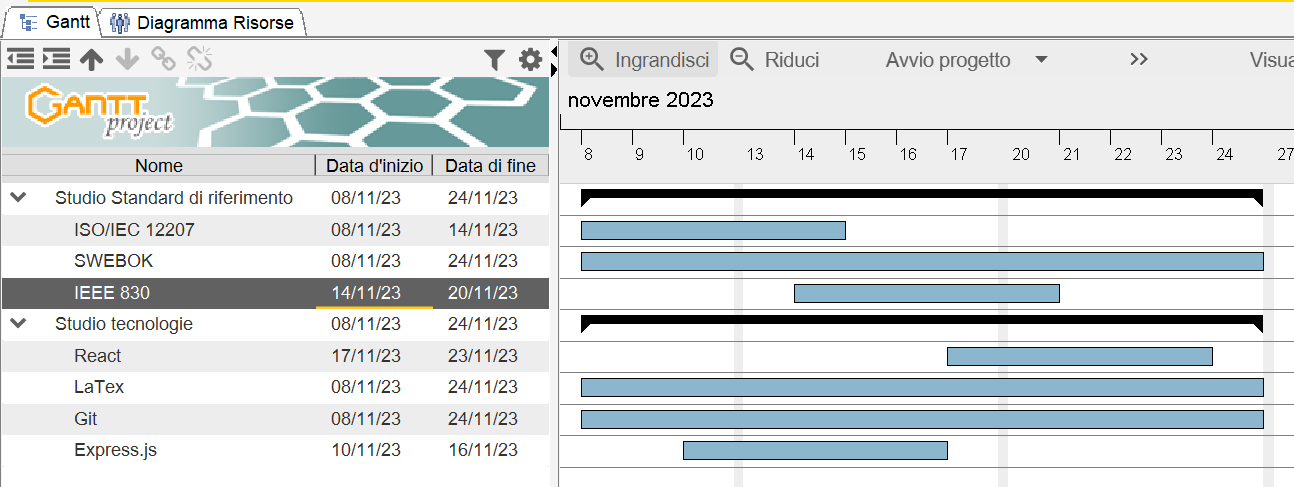
\includegraphics[scale=.6]{GanttPrimoPeriodo.png} \end{figure}

\textbf{Consuntivo orario}

\begin{tblr}{
    colspec={|X[5cm]|X[.5cm]|X[.5cm]|X[.5cm]|X[.5cm]|X[.5cm]|X[.5cm]|X[3.5cm]},
    row{odd}={bg=white},
    row{even}={bg=lightgray},
    row{1}={bg=black, fg=white},
    row{8}={bg=black, fg=white}
}

    Nominativo & Re & Am & An & Pg & Pr & Vf & Ore Totali \\ \hline
    Alberto C. & - & - & - & 4 & - & 1 & 5 \\ \hline
    Bilal El M. & - & - & 4 & - & - & 1 & 5 \\ \hline
    Alberto M. & 3 & 2 & - & - & - & - & 5 \\ \hline
    Alex S. & 2 & 3 & - & - & - & - & 5 \\ \hline
    Iulius S. & - & - & 4 & - & - & 1 & 5 \\ \hline
    Giovanni Z. & - & - & - & 4 & - & 1 & 5 \\ \hline
    Totale & 5 & 5 & 8 & 8 & 0 & 4 & 30 \\ \hline

\end{tblr}

\textbf{Consuntivo economico}

\begin{tblr}{
colspec={|X[5cm]|X[3.5cm]|X[1.5cm]|X[3.5cm]},
row{odd}={bg=white},
row{even}={bg=lightgray},
row{1}={bg=black, fg=white},
row{8}={bg=black, fg=white}
}

Ruolo & Costo orario (€/h) & N. Ore & Costo totale (€) \\ \hline
Responsabile & 30,00 & 5 & 150,00 \\ \hline
Amministratore & 20,00 & 5 & 100,00 \\ \hline
Analista & 25,00 & 8 & 200,00 \\ \hline
Progettista & 25,00 & 8 & 200,00 \\ \hline
Programmatore & 15,00 & 0 & 0,00 \\ \hline
Verificatore & 15,00 & 4 & 60,00 \\ \hline
Totale & \SetCell[c=1]{c} & 30 & 710,00 \\ \hline
\end{tblr}
\pagebreak

\textbf{Gestione dei ruoli}
\paragraph{}
In questo primo periodo, il 26\% delle ore di lavoro sono state dedicate alla fase di analisi,
data la necessità di effettuare uno studio preliminare dei documenti che dovranno essere prodotti durante
l'arco del progetto (in particolare le Norme di Progetto e il Piano di Progetto) e quindi dei relativi Standard internazionali di riferimento. \\
Un'eguale percentuale di risorse orarie è stata spesa per il ruolo di Progettista, per ricercare, individuare e studiare le tecnologie
potenzialmente adatte al prodotto da sviluppare; il 16\% delle ore è stato dedicato al ruolo del Responsabile, in cui si sono mossi i primi
passi nell'ambito della gestione ed organizzazione del carico di lavoro tra i vari membri; un'eguale percentuale di ore
è stata spesa per il ruolo di Amministratore il quale si è occupato dell'organizzazione della repository sulla piattaforma \emph{GitHub}$^{G}$.\\
Infine il 12\% delle ore è stato dedicato al ruolo di Verificatore,
durante le quali i membri hanno preso dimestichezza con l'operazione di verifica e validazione dei primi documenti prodotti.

\paragraph{Gestione dei rischi}

\begin{itemize}
\item \textbf{Rischio verificatosi:} Scarsa esperienza tecnologica:
\begin{itemize}
\item \textbf{Esito Piano di Contingenza:} Tramite lo studio individuale e soprattutto tramite la trasmissione di conoscenza dai membri maggiormente esperti nel linguaggio LaTex e nei comandi Git a quelli meno esperti, il gruppo è riuscito efficacemente a mettere in pratica il piano di contingenza previsto per il suddetto rischio, ottenendo un allineamento delle conoscenze tra i veri membri;
\item \textbf{Impatto:} L'impatto della scarsa esperienza tecnologica è stato nullo in questo primo periodo, avendo il gruppo preventivato la necessità di dedicare innanzitutto risorse all'individuazione, allo studio e all'apprendimento delle tecnologie di supporto, così come di quelle che andranno a far parte dello stack tecnologico del prodotto.
\end{itemize}
\end{itemize}

\paragraph{}
\textbf{Retrospettiva:}
In questo primo periodo, il gruppo ha speso la maggior parte delle proprie ore svolgendo un lavoro di ricerca ed analisi
su due fronti, ovvero quello della documentazione e del \emph{Proof of Concept}$^{G}$ (da cui in poi \emph{PoC}): Per quanto concerne la prima, sono stati studiati gli standard internazionali di riferimento
con lo scopo di disegnare una mappa concettuale dei documenti che dovranno essere prodotti, in particolare delle Norme ed del Piano di Progetto; per quanto
riguarda il PoC invece sono state individuate e studiate tecnologie potenzialmente adatte allo sviluppo del prodotto, e successivamente selezionate quelle utilizzate per il PoC stesso. \\
Inoltre, grande attenzione si è spesa per la definizione di norme che regolino il \emph{Way of Working}$^{G}$, data la presenza di studenti lavoratori (con
specifiche esigenze legate agli impegni extra-universitari) fra i membri del gruppo, e quindi la necessità di un'efficace ed efficiente gestione delle ore, della ripartizione dei ruoli
e della suddivisione dei task fra i membri stessi. Nonostante una buona definizione dei ruoli, il gruppo non è riuscito ancora ad individuare la modalità secondo la quale
ruotare in futuro i ruoli stessi.
\begin{itemize}
    \item \textbf{Obbiettivi raggiunti:}
    \begin{itemize}
        \item Allineamento da parte del gruppo, delle conoscenze del linguaggio LaTex e dei comandi Git;
        \item Scelta delle tecnologie da includere nello stack tecnologico;
        \item Inizio dell'analisi dei requisiti funzionali del prodotto.
    \end{itemize}\pagebreak
    \item \textbf{Obiettivi mancati:}
    \begin{itemize}
        \item Definizione della modalità di rotazione dei ruoli.
    \end{itemize}
\end{itemize}
